\documentclass{erciyes}

\usepackage{graphicx}
\usepackage{amsmath}
\usepackage{amssymb}
\usepackage{booktabs}
\usepackage{tabularx}
\usepackage{array}
\usepackage{float}
\usepackage{xcolor}
\usepackage{listings}
\usepackage{cite}
\usepackage{url}
\usepackage{tikz}
\usetikzlibrary{positioning,fit,arrows.meta}

% Henuz olculmemis degerler PDF'te kirmizi gorunsun; olculunce yerine sayi yazilir.
\newcommand{\olculecek}[1]{\textcolor{red}{\textbf{[ÖLÇÜLECEK: #1]}}}

\renewcommand{\thetable}{\arabic{table}}   % bölüm numarası kullanılmadığı için
\renewcommand{\thefigure}{\arabic{figure}}

% Türkçe kelimeler uzun olduğu için satırlar taşabiliyor;
% bu ayar kelimeler arasındaki boşluğu biraz esnetip taşmayı azaltıyor.
\setlength{\emergencystretch}{3em}

\ToCLineisDotted %% İçindekiler kısmında sayfa numaralarına kadar olan kısım noktalı olsun
\ToCChapterBold  %% İçindekiler kısmında BÖLÜM 1-2... yazıları bold olsun.
%\TabloListesiYok %% Tablo Listesi kullanılmayacak
%\SekilListesiYok %% Şekil Listesi kullanılmayacak

\setlength{\fboxsep}{0pt}

\newcommand{\plotPGFfile}{true} % PGF olarak DATA dosyaları çizilsin mi çizilmesin mi? Çizilmez ise dosyadan sadece data okunan kısım atlanıyor, resmin çerçevesi oluşturuluyor...
\definecolor{dkgreen}{rgb}{0,0.6,0}
\definecolor{gray}{rgb}{0.5,0.5,0.5}
\definecolor{mauve}{rgb}{0.58,0,0.82}

\lstset{frame=tb,
	language=Java, %Uygulamanın yazıldığı programlama dili, (Örnek kullanım chapter4.tex'te verilmiştir.)
	aboveskip=3mm,
	belowskip=3mm,
	showstringspaces=false,
	columns=flexible,
	basicstyle={\small\ttfamily},
	numbers=none,
	numberstyle=\tiny\color{gray},
	keywordstyle=\color{blue},
	commentstyle=\color{dkgreen},
	stringstyle=\color{mauve},
	breaklines=true,
	breakatwhitespace=true,
	tabsize=3
}

\author{Mustafa}{G{\"O}KTEPE}{1030510749}{1030510749@erciyes.edu.tr}{05331556738}%1. Öğrenci ad soyad
\authorIki{Ahmet}{ÇELİK}{1030510691}{1030510691@erciyes.edu.tr}{05453246440}%2. Öğrenci ad soyad Opsiyonel
\authorUc{Mustafa}{KÜPELİ}{1030510266}{1030510266@erciyes.edu.tr}{05360100620}%3. Öğrenci ad soyad  Opsiyonel
%\authorDort{Ad}{Soyad}{103051004}{numara4@erciyes.edu.tr}{054xxxxxxx}%4. Öğrenci ad soyad Opsiyonel

\anabilimdali{Bilgisayar Mühendisliği}
\anabilimdaliUpper{BİLGİSAYAR MÜHENDİSLİĞİ}

\date{Aralık 2026}
\Yil{2026-2027} %Eğitim Öğretim Yili
\Donem{Güz} %Donemi
\teziyoneten{Ar.\ G{\"O}r. HAYRİ ÖZTÜRK} % Tez Danismani





\title{MEDIAPIPE VE MAKİNE ÖĞRENMESİ KULLANARAK TÜRK İŞARET DİLİ (TİD) TABANLI GERÇEK ZAMANLI EL HAREKETİ TANIMA VE ÇEVİRİ SİSTEMİ} %TAMAMEN BÜYÜK HARF\vspace*{5mm}
\titleCase{MediaPipe ve Makine Öğrenmesi Kullanarak Türk İşaret Dili (TİD) Tabanlı Gerçek Zamanlı El Hareketi Tanıma ve Çeviri Sistemi} %Sadece ilk Harfleri Büyük




\renewcommand{\textfraction}{0.10}
\renewcommand{\topfraction}{0.95}
\renewcommand{\bottomfraction}{0.95}
\renewcommand{\floatpagefraction}{0.35}

\setcounter{totalnumber}{5}

\begin{document}
\clearpage
\section{Özet}
\label{CH:Ozet}

Bu projede, işitme engelli bireylerle işaret dili bilmeyen kişiler arasındaki iletişimi
kolaylaştırmak amacıyla, akıllı telefon kamerasından alınan Türk İşaret Dili (TİD)
kelimelerini tanıyıp yazıya çeviren bir Android uygulaması geliştirilmiştir. Sistem video
karesini değil, telefonda çıkarılan iskelet koordinatlarını kullanmaktadır. Bu sayede
internet bağlantısına ihtiyaç duyulmamakta ve kamera görüntüsü cihazdan dışarı
çıkmamaktadır.

Eğitim ve değerlendirmede AUTSL veri setinin işaretçiden bağımsız resmî bölmeleri
kullanılmıştır (226 işaret, 43 işaretçi). Her karede iki elin 21'er noktası ve üst gövdeye
ait 7 nokta Google MediaPipe Tasks ile çıkarılmış, koordinatlar omuz ortasına ötelenip
omuz genişliğine bölünmüş ve diziler 64 kareye örneklenmiştir. Aynı veri ve eğitim
düzeniyle iki model karşılaştırılmıştır: iki katmanlı, iki yönlü GRU (BiGRU, 2,11 milyon
parametre) ve 1B evrişim ile iki katmanlı Transformer kodlayıcısından oluşan model
(1B-CNN + Transformer, 1,47 milyon parametre). Üç farklı tohumla yapılan 60 epoch'luk
eğitimler sonunda 3.741 videoluk test kümesinde BiGRU yüzde $87{,}98 \pm 0{,}23$,
1B-CNN + Transformer yüzde $89{,}42 \pm 0{,}52$ Top-1 doğruluğa ulaşmış ve tez
önerisindeki yüzde 85 hedefini aşmıştır.

Seçilen 1B-CNN + Transformer modeli Keras üzerinden LiteRT biçimine aktarılmış ve
dinamik aralık int8 nicemleme uygulanmıştır. Model dosyası 1,61 MB'tır; test
doğruluğu nicemleme sonrası yüzde 89,82'dir ve PyTorch modeliyle tahminlerin yüzde
99,57'si aynıdır. Mobil uygulama Flutter ve Kotlin ile geliştirilmiştir: kamera,
MediaPipe ve model çıkarımı Kotlin tarafında çalışmakta, arayüz canlı tanıma, metin ve
işaret listesi olmak üzere üç ekrandan oluşmaktadır. İşaret listesinde her kelimenin
eğitim verisinden alınmış örnek hareketi iskelet animasyonu olarak gösterilmektedir.

Kaydedilmiş veri üzerinde hedefler sağlanırken iki konu açık kalmıştır. Uçtan uca hız,
iki MediaPipe modelinin kare başına çalışması nedeniyle 15 FPS hedefinin altındadır;
canlı kamera kullanımında ise tahmin güvenleri kayıtlı veriye göre düşmektedir. Bu iki
konuyu ölçmek ve ayrıştırmak için uygulamaya bir gönüllü testi ekranı ve kayıtları
bilgisayarda inceleyen bir analiz aracı eklenmiştir.

\vspace{3mm}
\noindent\textbf{Anahtar kelimeler:} Türk İşaret Dili, işaret dili tanıma, MediaPipe,
iskelet tabanlı tanıma, Transformer, çevrimdışı mobil uygulama, LiteRT.

\clearpage

\section{Giriş}
\label{CH:Giris}

\subsection{Problem ve motivasyon}

Türk İşaret Dili, işitme engelli bireylerin hem kendi aralarında hem de çevreleriyle
iletişim kurarken kullandığı doğal dildir~\cite{TIF2023}. İşaret dilini bilmeyen
kişilerle kurulan iletişim ise çoğu zaman yazı yazmaya ya da bir yakının
tercümanlığına bağlı kalmaktadır. Hastane, banka, okul ve resmî daire gibi ortamlarda
bu durum hem zaman kaybına hem de mahremiyet sorununa yol açmaktadır.

Projenin çıkış noktası, bu iletişim boşluğunda en yaygın cihazı, yani akıllı telefonu
kullanmaktır. Eldiven ya da derinlik kamerası gibi ek donanım gerektirmeyen bir çözüm
hem maliyeti düşürür hem de günlük kullanımda kabul edilebilirliği artırır. Sistemin
internet bağlantısına ihtiyaç duymaması, şebekenin zayıf olduğu yerlerde de
kullanılabilmesini ve kamera görüntüsünün cihazdan çıkmamasını sağlar.

\subsection{Amaç ve kapsam}

Projenin amacı, telefon kamerasının önünde yapılan bir TİD kelimesini tanıyıp yazıya
çeviren ve tamamen cihaz üzerinde çalışan bir Android uygulaması geliştirmektir.
Kapsam şu şekilde sınırlandırılmıştır:

\begin{itemize}
  \item Tanıma kelime düzeyindedir (izole işaret). Sözlük, AUTSL veri setindeki 226
        işaretle sınırlıdır.
  \item Art arda yapılan işaretler sürekli modda tek tek tanınıp yan yana yazılır;
        bunların dilbilgisel Türkçe cümleye çevrilmesi kapsam dışıdır.
  \item Parmak alfabesi (harf harf heceleme) veri setinde bulunmadığı için desteklenmez.
\end{itemize}

\subsection{Başarı ölçütleri}

Tez önerisinde belirlenen ölçütler Tablo~\ref{tab:olcutler} içinde verilmiştir. Bu
ölçütlerin hangilerinin sağlandığı Bölüm~\ref{CH:Degerlendirme} içinde
tartışılmaktadır.

\begin{table}[H]
\centering
\caption{Tez önerisindeki değerlendirme ölçütleri ve hedefler}
\label{tab:olcutler}
\begin{tabular}{@{}lll@{}}
\toprule
\textbf{Ölçüt} & \textbf{Ölçüm ortamı} & \textbf{Hedef} \\
\midrule
Top-1 doğruluk & AUTSL test kümesi & $\geq$ yüzde 85 \\
Gerçek ortam doğruluğu & Gönüllü testi (30 işaret) & $\geq$ yüzde 75 \\
Model boyutu & \texttt{.tflite} dosyası & $\leq$ 10 MB \\
İşleme hızı & Orta segment Android telefon & $\geq$ 15 kare/s \\
İnternet bağımlılığı & Uçak modu & Tam çalışma \\
\bottomrule
\end{tabular}
\end{table}

\subsection{Ekip ve iş bölümü}

Proje üç kişilik bir ekip tarafından yürütülmüştür. Her alanın bir sorumlusu
belirlenmiş, ancak veri, model ve uygulama aynı hattın parçaları olduğu için kararlar
birlikte alınmıştır: veri hazırlığı, veri hattı ve normalizasyon (Mustafa Küpeli);
yapay zekâ modeli, eğitim ve optimizasyon (Mustafa Göktepe); mobil uygulama, kullanıcı
arayüzü ve donanım entegrasyonu (Ahmet Çelik). Çalışma ortak bir Git deposunda
yürütülmüş, her deney \texttt{experiments/} klasöründe tarih, tohum ve sonuçlarıyla
kaydedilmiştir.

\subsection{Tezin düzeni}

Bölüm~\ref{CH:Literatur} işaret dili tanıma alanındaki çalışmaları ve Türk İşaret Dili
veri setlerini özetlemektedir. Bölüm~\ref{CH:Veri} veri setini ve ön işlemeyi,
Bölüm~\ref{CH:Model} model mimarilerini, eğitimi ve hata analizini anlatmaktadır.
Bölüm~\ref{CH:Uygulama} modelin telefona aktarılmasını ve mobil uygulamayı,
Bölüm~\ref{CH:Degerlendirme} başarı ölçütlerine göre değerlendirmeyi içermektedir.
Bölüm~\ref{CH:Sonuc} sonuçları ve gelecek çalışmaları özetlemektedir.

\section{Literatür ve Veri Setleri}
\label{CH:Literatur}

\subsection{İşaret dili tanıma yaklaşımları}

İzole işaret dili tanımada iki ana yaklaşım bulunmaktadır. Görüntü tabanlı
yöntemler video karelerini doğrudan evrişimli ya da üç boyutlu evrişimli ağlarla
işler. Bu yöntemler yüksek doğruluk verse de büyük modeller ve güçlü donanım
gerektirir; çoğunlukla sunucu tarafında çalıştırılır. İskelet tabanlı yöntemler ise
önce her karede el, yüz ve gövde noktalarını çıkarır, sınıflandırmayı bu koordinat
dizileri üzerinde yapar. Girdi boyutu çok küçük olduğu için modeller hafif kalır ve
kişinin görünüşü, arka plan ya da ışık gibi etkenlerden daha az etkilenir.

AUTSL veri setinin yayımlandığı çalışmada RGB ve derinlik verisi üzerinde CNN ile
LSTM birleşimi temel yöntem olarak sunulmuştur~\cite{AUTSL2020}. Aynı veri setiyle
düzenlenen ChaLearn LAP 2021 yarışmasında işaretçiden bağımsız değerlendirme
yapılmış, en iyi sonuçlar birden fazla modaliteyi (RGB, derinlik, iskelet) birleştiren
yöntemlerle alınmıştır~\cite{ChaLearn2021}. Bu yöntemlerden SAM-SLR, iskelet
noktalarını çizge evrişimli ağlarla işleyerek diğer modalitelerle
birleştirmiştir~\cite{SAMSLR2021}. Yarışmanın ilk sıraları yüzde 98 civarında test
doğruluğuna ulaşmış, ancak bu sonuçlar büyük model toplulukları ve tam video girdisiyle
elde edilmiştir; telefonda gerçek zamanlı çalışma hedeflenmemiştir.

Mobil cihaz hedefli çalışmalarda Google'ın Kaggle üzerinde düzenlediği Amerikan
İşaret Dili yarışması öne çıkmaktadır~\cite{KaggleASL2023}. Bu yarışmada girdiler
MediaPipe ile çıkarılmış nokta dizileridir ve modellerin TensorFlow Lite biçiminde,
sınırlı boyut ve sürede çalışması şart koşulmuştur. Öne çıkan çözümlerde nokta
dizileri üzerinde 1B evrişim ve küçük Transformer katmanları kullanılmıştır. Bu
projede karşılaştırılan ikinci mimari bu yaklaşımdan esinlenmiştir.

TİD üzerine iskelet tabanlı çalışmalar da son yıllarda artmaktadır. TSLFormer,
AUTSL üzerinde MediaPipe noktalarını kullanan hafif bir Transformer
önermiştir~\cite{TSLFormer2025}. Torun ve Karacı, MediaPipe Holistic noktalarıyla 41
TİD ifadesi üzerinde GRU, LSTM ve bunların birleşimlerini
karşılaştırmıştır~\cite{Torun2024}.

\subsection{Nokta çıkarımı: MediaPipe}

MediaPipe, Google'ın cihaz üzerinde çalışan algılama hatları için geliştirdiği bir
çerçevedir~\cite{MediaPipe2019}. El modeli önce avuç içini bulur, ardından her el için
21 nokta üretir~\cite{MediaPipeHands2020}. Gövde modeli (BlazePose) 33 nokta
üretir~\cite{BlazePose2020}. Bu projede yeni \textit{Tasks} arayüzündeki
\texttt{hand\_landmarker} ve \texttt{pose\_landmarker\_lite} modelleri kullanılmıştır.
Aynı modellerin hem Python'da (eğitim verisinin çıkarımı) hem Android'de (canlı
kullanım) bulunması, eğitim ile uygulama arasındaki nokta sırası ve ölçek farklarını
ortadan kaldırmak için belirleyici olmuştur.

\subsection{Türk İşaret Dili veri setleri}

Proje başında ve sonunda yapılan taramalarda bulunan kelime düzeyindeki TİD veri
setleri Tablo~\ref{tab:verisetleri} içinde özetlenmiştir.

\begin{table}[H]
\centering
\caption{Kelime düzeyindeki Türk İşaret Dili veri setleri}
\label{tab:verisetleri}
\small
\begin{tabularx}{\textwidth}{@{}l r r r X@{}}
\toprule
\textbf{Veri seti} & \textbf{İşaret} & \textbf{İşaretçi} & \textbf{Video} & \textbf{Erişim} \\
\midrule
AUTSL~\cite{AUTSL2020} & 226 & 43 & 36.302 & Akademik kullanım; bu projede kullanıldı \\
BosphorusSign22k~\cite{Bosphorus2020} & 744 & 6 & 22.542 & Yazarlara lisans sözleşmesi gönderilerek \\
TurkSign446~\cite{TurkSign446} & 446 & 10 & 44.600 & Dosyalar kısıtlı, erişim talebiyle; yalnızca MediaPipe noktaları \\
\bottomrule
\end{tabularx}
\end{table}

AUTSL, işaretçi sayısının fazlalığı ve resmî bölmelerinin işaretçiden bağımsız olması
nedeniyle ana veri seti olarak seçilmiştir. Altı işaretçili BosphorusSign22k ve on
katılımcılı TurkSign446 daha geniş sözlük sunmakla birlikte kişi çeşitliliği daha
düşüktür; ikisi de erişim izni gerektirdiği için bu dönemde kullanılamamıştır. Bu veri
setleriyle sözlüğün genişletilmesi gelecek çalışma olarak bırakılmıştır.

\subsection{Projenin farkı}

Literatürdeki yüksek doğruluklu çalışmaların önemli bir kısmı sunucuda çalışan büyük
modellere dayanmaktadır. Bu projenin katkısı modelin kendisinden çok, hattın uçtan uca
ve telefonda çalışmasındadır:

\begin{itemize}
  \item Girdi olarak video karesi değil iskelet koordinatları kullanılmış, model 1,6 MB
        ile sınırlı tutulmuştur. Ham görüntü işlenmediği için kişisel veri yükü azalmıştır.
  \item Nokta çıkarımı eğitimde ve telefonda aynı MediaPipe Tasks modelleriyle
        yapılmış, ön işleme Python ve Kotlin'de birebir aynı yazılmıştır. Aynı 200 örnekte
        iki taraf yüzde 99,5 oranında aynı tahmini vermektedir.
  \item Sistem tamamen çevrimdışıdır; uygulamanın internet izni bulunmamaktadır.
  \item Kullanıcının işareti doğru yapabilmesi için her kelimenin örnek hareketi
        uygulama içinde iskelet animasyonu olarak gösterilmektedir.
\end{itemize}

\section{Veri Seti ve Ön İşleme}
\label{CH:Veri}

\subsection{AUTSL veri seti}

Çalışmada AUTSL veri seti kullanılmıştır~\cite{AUTSL2020}. Veri setinde 226 işaret,
43 işaretçi ve toplam 36.302 video bulunmaktadır. Videolar 512$\times$512 çözünürlükte
ve saniyede 30 karedir. Resmî bölmeler \texttt{train} (28.142 video, 31 işaretçi),
\texttt{val} (4.418 video, 6 işaretçi) ve \texttt{test} (3.742 video, 6 işaretçi)
şeklindedir. Bölmeler arasında ortak işaretçi bulunmadığı ve sınıf numaralarının üç
bölmede de aynı anlama geldiği ayrıca kontrol edilmiştir. Böylece ölçülen doğruluk,
modelin daha önce görmediği kişiler üzerindeki başarısını göstermektedir.

Kaggle üzerinden indirilen kopyada 11 videonun açılamadığı görülmüştür. Bu dosyalarda
MP4 kutusuna ait \texttt{moov} bilgisi eksiktir, yani dosyalar yarım inmiştir. İlgili
videolar atlanmış, kalan 28.132 eğitim, 4.418 doğrulama ve 3.741 test videosu ile
çalışılmıştır. Sınıf numarası ile Türkçe kelime eşlemesi
\texttt{SignList\_ClassId\_TR\_EN.csv} dosyasından okunmakta, uygulamada kelimeler
Türkçe yazımıyla (örneğin \sol cikmak\sag{} yerine \sol çıkmak\sag) gösterilmektedir.

\subsection{Nokta çıkarımı}

Her video karesi MediaPipe Tasks API'ye video modunda verilmiş, iki el için 21'er nokta
ve üst gövde için 7 nokta (burun, iki omuz, iki dirsek, iki bilek) alınmıştır. Tüm veri
setinin çıkarımı tek bir bilgisayarda yapılmış, sonuçlar her video için bir
\texttt{.npz} dosyası olarak saklanmıştır (toplam 1,1 GB). Ellerin bulunma oranı sol
elde yüzde 82, sağ elde yüzde 86 olarak ölçülmüş, gövde noktaları tüm karelerde
yakalanmıştır. Elin bulunmadığı karelerde ilgili koordinatlar sıfırlanmakta ve iki
boyutlu bir \sol el var mı\sag{} göstergesi özellik vektörüne eklenmektedir.

MediaPipe'ın sol/sağ el etiketi, gövde modelinin sol ve sağ bilek noktalarıyla
karşılaştırılmış ve 28.689 el-karede yüzde 98 oranında uyumlu bulunmuştur. AUTSL
videoları aynalanmamıştır; telefondaki analiz görüntüsü de aynalanmadan işlenmektedir.

\subsection{Normalizasyon ve sabit uzunluk}

Kişinin kameraya uzaklığı ve boyu modeli etkilemesin diye her karedeki noktalar iki
omzun orta noktasına göre ötelenmiş ve omuz genişliğine bölünmüştür:
\begin{equation}
  \hat{p}_i = \frac{p_i - \tfrac{1}{2}(s_{\text{sol}} + s_{\text{sağ}})}{\lVert s_{\text{sol}} - s_{\text{sağ}} \rVert}
\end{equation}
Burada $p_i$ bir noktanın görüntü koordinatı, $s$ ise omuz noktalarıdır. Omuzların
bulunamadığı karelerde bir önceki geçerli değer kullanılmaktadır. Telefon görüntüsü
kare olmadığı için Kotlin tarafında koordinatlar önce piksel birimine çevrilmekte,
böylece eğitimdeki kare görüntüyle ölçek farkı ortadan kalkmaktadır.

Normalizasyondan sonra her kare
$2\times21\times2 + 7\times2 + 2 = 100$ boyutlu bir vektörle temsil edilmektedir
(koordinatlar $x$ ve $y$; derinlik kullanılmamıştır). Videoların uzunluğu değişken
olduğu için (eğitim kümesinde ortalama yaklaşık 60 kare) her dizi doğrusal
interpolasyonla 64 kareye örneklenmektedir. Modelin girdisi bu nedenle
$64\times100$ boyutludur.

\subsection{Veri artırma}

Eğitimde dört tür artırma uygulanmaktadır. En önemlisi zamansal seyreltmedir: kareler
rastgele 1, 2 veya 3 adımda bir alınarak 30, 15 ve 10 FPS'lik kayıtlara benzetilir.
Bunun nedeni telefon kamerasının gerçek kullanımda saniyede yaklaşık 9--12 kare
işleyebilmesidir. Diğer artırmalar dizinin iki ucundan yüzde 10'a kadar kırpma,
$\pm10^\circ$ döndürme, yüzde 90--110 arası ölçek değişimi ve küçük bir kaydırmadır.
Artırma yalnızca eğitim kümesine uygulanmaktadır.

\section{Model ve Eğitim}
\label{CH:Model}

\subsection{BiGRU temel modeli}

Temel sınıflandırıcı olarak iki katmanlı ve iki yönlü bir GRU (BiGRU) kurulmuştur~\cite{Cho2014}.
Girdi önce 100 boyuttan 256 boyuta indirgenir (doğrusal katman, ReLU, yüzde 20
dropout). Ardından iki GRU katmanı diziyi ileri ve geri yönde işler. Çıkışta son gizli
durum yerine zaman ekseni boyunca ortalama alınır ve 226 sınıfa yönelik doğrusal katman
uygulanır. Zaman ortalamasının seçilme nedeni, işaretin hangi karede bittiğinin kesin
olmaması ve dizinin başındaki ya da sonundaki boş karelerin sonucu kaydırmasının
istenmemesidir. Modelin katmanları Tablo~\ref{tab:gru} içinde verilmiştir.

\begin{table}[H]
\centering
\caption{BiGRU modelinin katmanları ve parametre sayıları}
\label{tab:gru}
\begin{tabular}{lrr}
\toprule
\textbf{Katman} & \textbf{Çıkış boyutu} & \textbf{Parametre} \\
\midrule
Girdi doğrusal katmanı & $64\times256$ & 25.856 \\
GRU katmanı 1 (iki yönlü) & $64\times512$ & 787.968 \\
GRU katmanı 2 (iki yönlü) & $64\times512$ & 1.181.184 \\
Çıkış doğrusal katmanı & 226 & 115.938 \\
\midrule
\textbf{Toplam} & & \textbf{2.114.018} \\
\bottomrule
\end{tabular}
\end{table}

\subsection{1B-CNN + Transformer modeli}

İkinci mimari, üç katmanlı 1B evrişim ağı ile iki katmanlı Transformer
kodlayıcısının~\cite{Vaswani2017} birleşimidir. Evrişim katmanları
($100\rightarrow128\rightarrow256\rightarrow256$, her birinden sonra batch
normalizasyonu ve GELU) kısa süreli yerel el hareketlerini çıkarır. İkinci evrişim
katmanındaki 2 adımlık kaydırma dizi uzunluğunu 64'ten 32'ye indirerek sonraki dikkat
hesabının maliyetini düşürür. Sinüzoidal konum kodlamasının ardından gelen Transformer
kodlayıcısı ($d_{\text{model}}=256$, 4 dikkat başlığı, ileri besleme boyutu 512, ön
normalizasyon) uzun menzilli zaman ilişkilerini öğrenir. Çıkışta yine zaman ortalaması
alınır, katman normalizasyonundan sonra 226 sınıfa doğrusal katman uygulanır. Model
1.473.634 parametreye sahiptir, yani BiGRU'dan yaklaşık yüzde 30 daha küçüktür. Ayrıca
tekrarlayan katman içermediği için eğitimi paralelleştirilebilir.

\subsection{Eğitim düzeni}

Her iki model de PyTorch ile aynı veri, aynı artırma ve aynı hiperparametrelerle
eğitilmiştir: 60 epoch, AdamW~\cite{Loshchilov2019} ($\text{lr}=2\times10^{-3}$,
ağırlık azaltımı $10^{-2}$), kosinüs öğrenme oranı azaltımı, 128'lik batch ve 0,1
etiket yumuşatma~\cite{Szegedy2016}. Doğrulama doğruluğu en yüksek olan epoch'un
ağırlıkları saklanmış, test kümesi yalnızca eğitim bittikten sonra bir kez ölçülmüştür.
Tek bir koşunun şans eseri iyi ya da kötü çıkabileceği göz önüne alınarak her model
üç farklı tohumla (0, 1, 2) eğitilmiştir. Eğitimler Apple M4 (MPS) ve NVIDIA RTX 3050
üzerinde yapılmış, tohum 0 için 60 epoch BiGRU'da 77,6 dakika, 1B-CNN + Transformer'da
18,1 dakika sürmüştür.

Kodda veri hazırlığı (\texttt{features.py}), modeller (\texttt{models.py}) ve eğitim
döngüsü (\texttt{train\_gru.py}) ayrı dosyalardadır. Her koşu
\texttt{experiments/} altına tohum, hiperparametreler, epoch bazında kayıp ve
doğrulama doğruluğu ile birlikte JSON olarak yazılmaktadır.

\subsection{Sonuçlar}

Tohum 0 ile yapılan karşılaştırma Tablo~\ref{tab:tohum0}, üç tohumun ortalaması ve
standart sapması Tablo~\ref{tab:uctohum} içinde verilmiştir. Eğitim kaybı ve doğrulama
doğruluğunun epoch'lara göre değişimi Şekil~\ref{fig:egri} üzerinde görülmektedir.

\begin{table}[H]
\centering
\caption{226 sınıfta iki modelin karşılaştırması (tohum 0, 60 epoch)}
\label{tab:tohum0}
\small
\begin{tabular}{@{}lrrrr@{}}
\toprule
\textbf{Model} & \textbf{Parametre} & \textbf{Doğrulama (\%)} & \textbf{Test (\%)} & \textbf{Macro F1 (\%)} \\
\midrule
BiGRU-2x256 & 2.114.018 & 89,23 & 88,24 & 88,09 \\
1B-CNN + Transformer & 1.473.634 & \textbf{89,97} & \textbf{88,83} & \textbf{88,61} \\
\bottomrule
\end{tabular}
\end{table}

\begin{table}[H]
\centering
\caption{Üç tohumla (0, 1, 2) test ve doğrulama doğrulukları}
\label{tab:uctohum}
\small
\setlength{\tabcolsep}{4pt}
\begin{tabular}{@{}lccc|cc@{}}
\toprule
\textbf{Model} & \textbf{Tohum 0} & \textbf{Tohum 1} & \textbf{Tohum 2} & \textbf{Test ort.\ $\pm$ ss} & \textbf{Doğr.\ ort.} \\
\midrule
BiGRU-2x256 & 88,24 & 87,81 & 87,89 & 87,98 $\pm$ 0,23 & 89,38 \\
1B-CNN + Transformer & 88,83 & 89,79 & 89,66 & \textbf{89,42 $\pm$ 0,52} & \textbf{90,37} \\
\bottomrule
\end{tabular}
\end{table}

\begin{figure}[H]
\centering
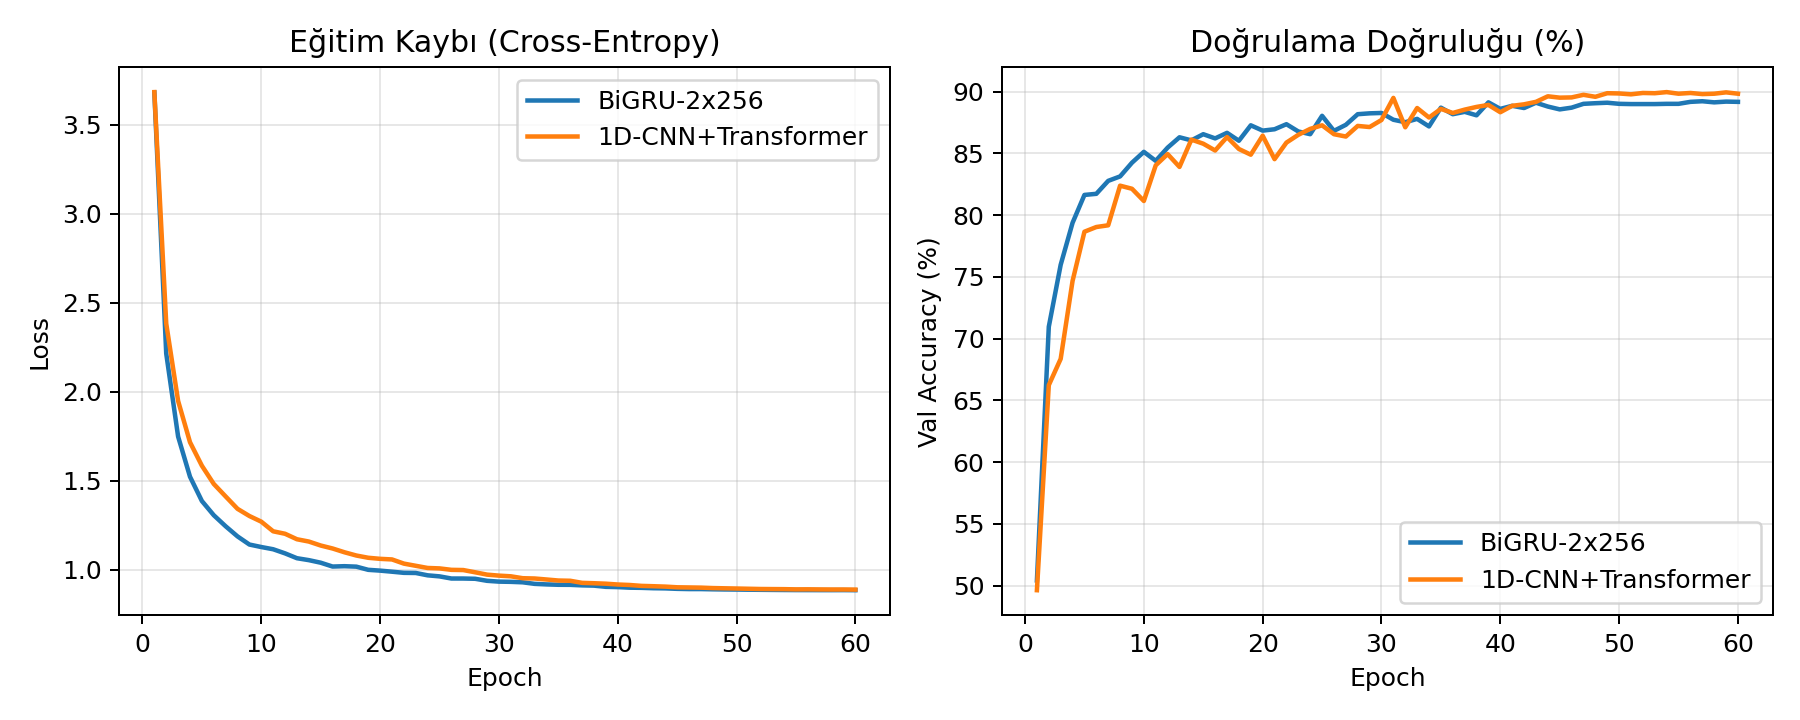
\includegraphics[width=0.95\textwidth]{grafik/egitim_egrisi.png}
\caption{İki modelin 60 epoch boyunca eğitim kaybı ve doğrulama doğruluğu (tohum 0)}
\label{fig:egri}
\end{figure}

1B-CNN + Transformer modeli üç tohumun üçünde de BiGRU'dan daha yüksek test
doğruluğuna ulaşmış, ortalamada fark yaklaşık 1,4 puan olmuştur. Şekil~\ref{fig:egri}
incelendiğinde BiGRU'nun ilk epoch'larda daha hızlı yükseldiği, ancak 30. epoch'tan
sonra Transformer tabanlı modelin öne geçtiği görülmektedir. Daha az parametreye sahip
olması, eğitiminin daha hızlı olması ve telefonda da daha küçük kalması
(Bölüm~\ref{CH:Uygulama}) nedeniyle uygulamada kullanılacak model olarak
1B-CNN + Transformer seçilmiş, üç tohum içinde doğrulama doğruluğu en yüksek olan
tohum 1 ağırlıkları alınmıştır (doğrulama yüzde 90,56, test yüzde 89,79).

\subsection{Hata analizi}

Hataların nerede toplandığını görmek için test kümesindeki 3.741 örnek üzerinde
karışıklık matrisi ve sınıf bazlı F1 skorları çıkarılmıştır
(\texttt{error\_analysis.py}). En çok karışan 18 sınıfın alt matrisi
Şekil~\ref{fig:cm}, en sık karışan işaret çiftleri Tablo~\ref{tab:karisan} içinde
verilmiştir.

\begin{figure}[H]
\centering
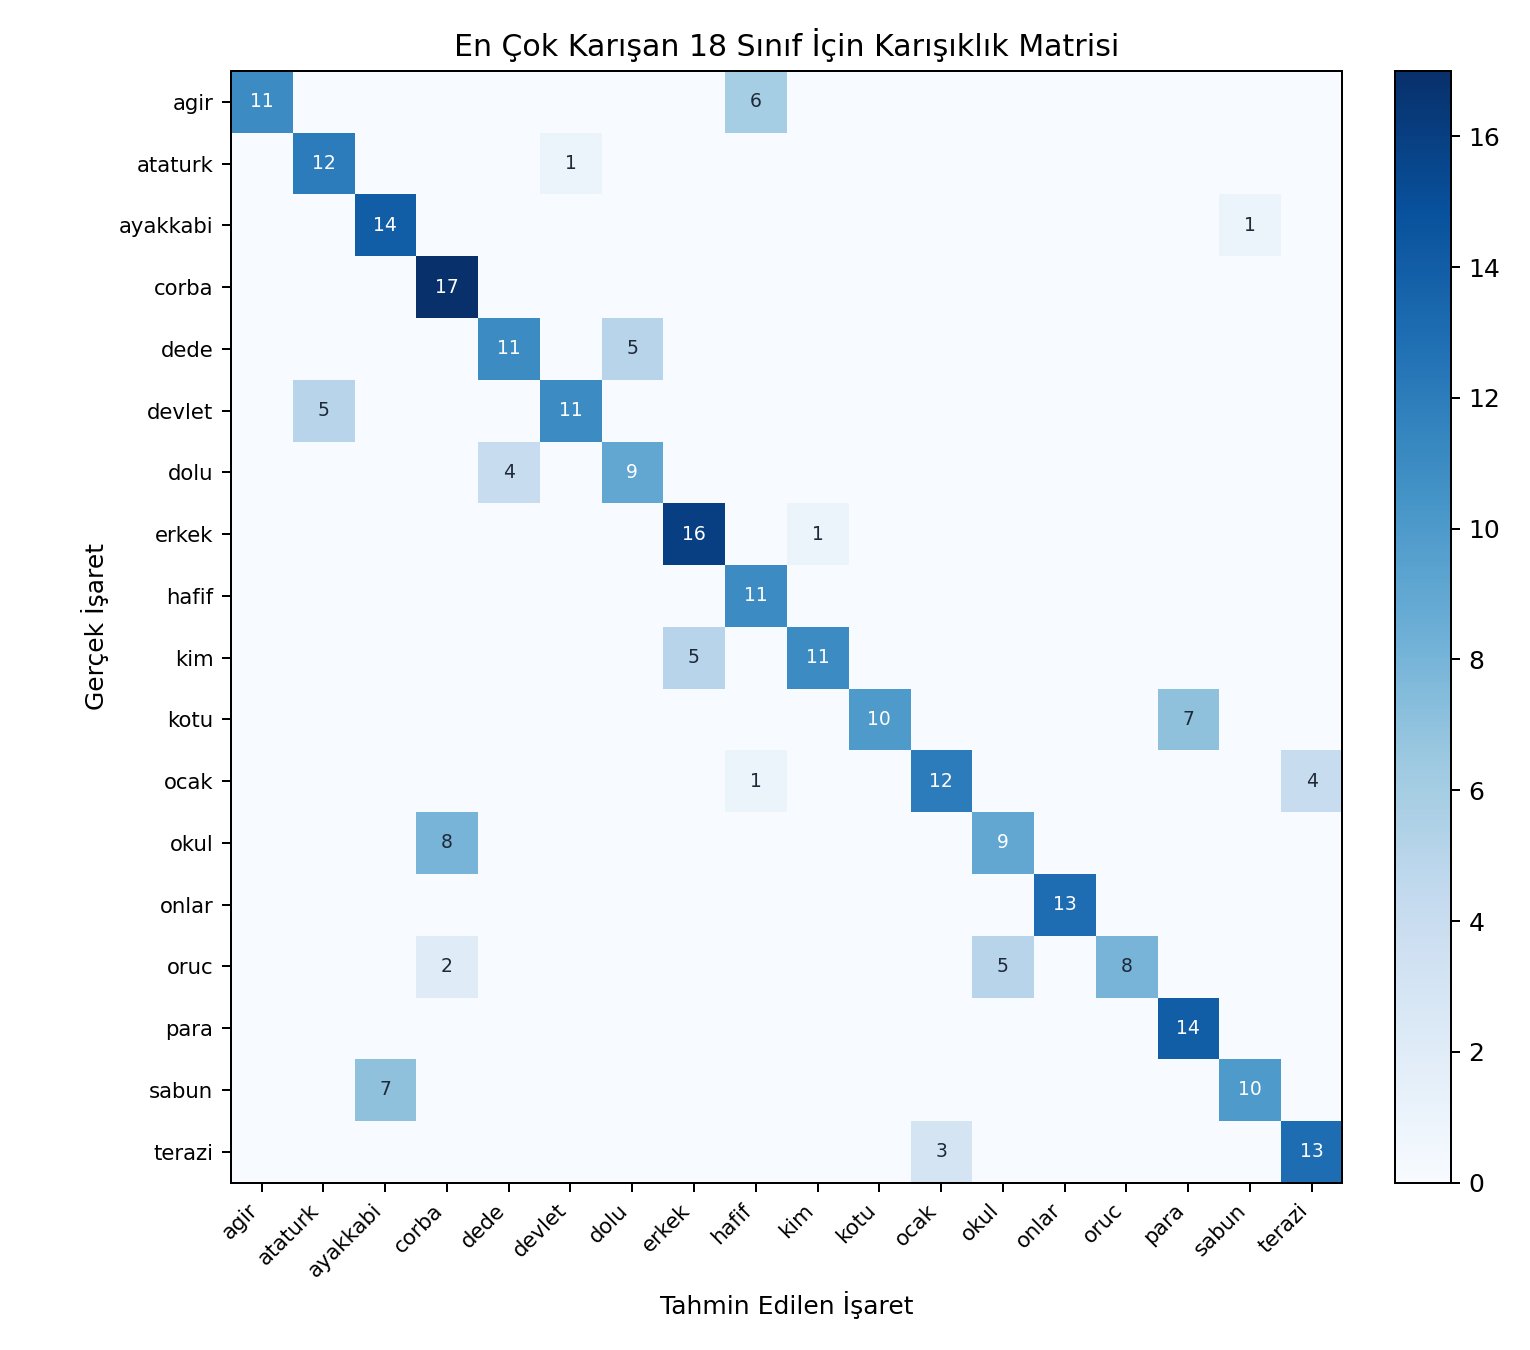
\includegraphics[width=0.8\textwidth]{grafik/karisiklik_matrisi.png}
\caption{Test kümesinde en çok karışan 18 sınıf için karışıklık matrisi (1B-CNN + Transformer, tohum 0)}
\label{fig:cm}
\end{figure}

\begin{table}[H]
\centering
\caption{Test kümesinde en sık karışan işaret çiftleri}
\label{tab:karisan}
\small
\begin{tabularx}{\textwidth}{@{}l l r X@{}}
\toprule
\textbf{Gerçek} & \textbf{Tahmin} & \textbf{Hata / Toplam} & \textbf{Olası neden} \\
\midrule
okul & çorba & 8 / 17 & İki elin göğüs önünde benzer kavisli hareketi \\
kötü & para & 7 / 17 & Parmak ucu sürtme hareketinin iki boyutta benzemesi \\
sabun & ayakkabı & 7 / 17 & İki elin birbirine sürtünme hareketi \\
ağır & hafif & 6 / 17 & Aynı el biçimi, yalnızca zıt yönde (aşağı/yukarı) hareket \\
oruç & okul & 5 / 16 & Ağız hizasında başlayan benzer el konumu \\
\bottomrule
\end{tabularx}
\end{table}

Hatalar rastgele dağılmamakta, el biçimi ve konumu aynı olup yalnızca ince parmak
teması ya da derinlik yönündeki hareketle ayrışan işaretlerde toplanmaktadır. En düşük
F1 skoruna sahip sınıflar \sol doktor\sag, \sol perşembe\sag, \sol dakika\sag{} ve
\sol yastık\sag{} olmuştur (F1 yüzde 48--54). Bu işaretlerin ayırt edici bilgisi
çoğunlukla parmakların yüze ya da birbirine değmesinde bulunmakta ve iki boyutlu
koordinatlarda zayıf kalmaktadır.

\subsection{Güven eşiği}

Model, sözlükte olmayan ya da yarım kalmış bir hareketi de 226 sınıftan birine atar. Bu
tür tahminleri ayıklamak için en yüksek softmax olasılığı üzerinde bir güven eşiği
uygulanmaktadır. Eşik, doğrulama kümesinde seçilip test kümesinde kontrol edilmiştir
(\texttt{calibrate\_threshold.py}). Uygulamadaki model için sonuçlar
Tablo~\ref{tab:esik} içindedir.

\begin{table}[H]
\centering
\caption{Güven eşiğine göre kabul oranı ve kabul edilenlerde doğruluk (1B-CNN + Transformer, test kümesi)}
\label{tab:esik}
\begin{tabular}{@{}rrr@{}}
\toprule
\textbf{Eşik} & \textbf{Kabul edilen (\%)} & \textbf{Kabul edilenlerde doğruluk (\%)} \\
\midrule
0 & 100,0 & 89,8 \\
0,5 & 88,7 & 95,0 \\
0,6 & 85,4 & 96,1 \\
0,7 & 80,2 & 97,0 \\
0,8 & 71,3 & 97,8 \\
\bottomrule
\end{tabular}
\end{table}

Uygulamada varsayılan eşik 0,6'dır ve kullanıcı ayarlardan değiştirebilir. Bu eşikte
test örneklerinin yüzde 85,4'ü kabul edilmekte ve bunlarda doğruluk yüzde 96,1'e
çıkmaktadır. Aynı eşikte BiGRU modeli örneklerin ancak yüzde 75'ini kabul
etmektedir. Elin hiç görünmediği yapay girdilerde modelin yine de bir kelime seçtiği
görüldüğünden, uygulamada kayıt boyunca el karelerin beşte birinden azında görünmüşse
kayıt modele verilmeden kullanıcı uyarılmaktadır.

\section{Mobil Uygulama}
\label{CH:Uygulama}

\subsection{Modelin telefona aktarılması}

Eğitilen modeller LiteRT (\texttt{.tflite}) biçimine dönüştürülmüştür~\cite{LiteRT}.
PyTorch'tan doğrudan dönüşüm aracı (\texttt{ai-edge-torch}) eğitim bilgisayarına
kurulamadığı için modeller Keras'ta aynı katmanlarla yeniden kurulmuş ve ağırlıklar
birebir taşınmıştır. BiGRU'da PyTorch'un kapı sırası $(r, z, n)$ Keras'ın $(z, r, h)$
sırasına çevrilmiştir. 1B-CNN + Transformer'da ise şu farklara dikkat edilmiştir:
evrişim ağırlıklarının eksen sırası, 2 adımlı evrişimde Keras'ın \texttt{same} dolgusunun
sağa fazladan sıfır eklemesi (açık dolgu ve \texttt{valid} ile çözülmüştür), normalizasyon
katmanlarının epsilon değeri ($10^{-5}$) ve GELU'nun tam (erf) sürümü. Keras ile PyTorch
çıktıları arasındaki en büyük fark $7\times10^{-6}$ olarak ölçülmüştür.

Dönüştürülen modellere dinamik aralık int8 nicemleme uygulanmıştır: ağırlıklar 8 bit
saklanmakta, hesaplamalar kayan noktada yapılmaktadır. Sonuçlar
Tablo~\ref{tab:donusum} içinde verilmiştir.

\begin{table}[H]
\centering
\caption{LiteRT dönüşümü sonrası boyut ve test doğruluğu (3.741 test videosu; son sütun PyTorch modeliyle aynı tahmin oranı)}
\label{tab:donusum}
\small
\begin{tabular}{@{}llrrr@{}}
\toprule
\textbf{Model} & \textbf{Biçim} & \textbf{Boyut (MB)} & \textbf{Test (\%)} & \textbf{Aynı tahmin (\%)} \\
\midrule
BiGRU & fp32 & 9,43 & 88,00 & 100,0 \\
BiGRU & int8 & 3,19 & 88,00 & 99,5 \\
1B-CNN + Transformer & fp32 & 5,95 & 89,79 & 100,0 \\
1B-CNN + Transformer & int8 & \textbf{1,61} & \textbf{89,82} & 99,6 \\
\bottomrule
\end{tabular}
\end{table}

Nicemleme doğruluğu düşürmemiş, 1B-CNN + Transformer modelinin int8 sürümü BiGRU'nun
yarısı boyutunda kalmıştır. Uygulamada bu sürüm kullanılmaktadır.

\subsection{Mimari}

Uygulama Flutter ile yazılmış, kamera ve hesaplama işleri Kotlin tarafında
tutulmuştur (Şekil~\ref{fig:mimari}). Her kareyi Flutter ile Kotlin arasında taşımak
kare hızını belirgin biçimde düşüreceği için kamera görüntüsü, MediaPipe ve model
çıkarımı tamamen Kotlin'de çalışmaktadır. Flutter tarafına yalnızca yarım saniyede bir
özet bilgiler (kare hızı, görünen el sayısı) ve tanıma sonuçları olay kanalı
(\textit{event channel}) üzerinden gelmektedir.

\begin{figure}[H]
\centering
\resizebox{\textwidth}{!}{%
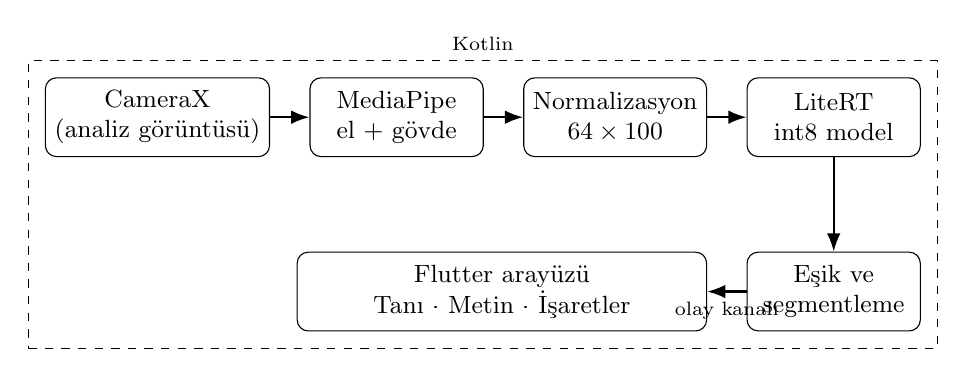
\begin{tikzpicture}[
  kutu/.style={draw, rounded corners, align=center, minimum height=1.0cm, minimum width=2.2cm, font=\small},
  ok/.style={-{Latex}, thick}]
\node[kutu] (kam) {CameraX\\(analiz görüntüsü)};
\node[kutu, right=0.5cm of kam] (mp) {MediaPipe\\el + gövde};
\node[kutu, right=0.5cm of mp] (on) {Normalizasyon\\$64\times100$};
\node[kutu, right=0.5cm of on] (lr) {LiteRT\\int8 model};
\node[kutu, below=1.2cm of lr] (seg) {Eşik ve\\segmentleme};
\node[kutu, left=0.5cm of seg, minimum width=5.2cm] (fl) {Flutter arayüzü\\Tanı · Metin · İşaretler};
\draw[ok] (kam) -- (mp);
\draw[ok] (mp) -- (on);
\draw[ok] (on) -- (lr);
\draw[ok] (lr) -- (seg);
\draw[ok] (seg) -- node[below, font=\scriptsize]{olay kanalı} (fl);
\node[draw, dashed, fit=(kam)(mp)(on)(lr)(seg), inner sep=6pt, label={[font=\scriptsize]above:Kotlin}] {};
\end{tikzpicture}}
\caption{Uygulamanın veri akışı. Kesikli çerçevedeki adımlar Kotlin tarafında çalışır.}
\label{fig:mimari}
\end{figure}

El ve gövde modelleri ayrı iş parçacıklarında paralel çalışmaktadır. El modeli
grafik işlemcide (GPU), gövde modeli merkezi işlemcide (CPU) çalıştırıldığında en
yüksek kare hızı alınmıştır. Gövde noktaları yavaş değiştiği için her iki karede bir
çıkarılmakta, aradaki karede son değer kullanılmaktadır. Bu değişikliğin doğruluğa
etkisi AUTSL test kümesinde 10 FPS'e seyreltilmiş videolarla ölçülmüş, her karede
çıkarımla iki karede bir çıkarım arasında fark görülmemiştir (ikisinde de yüzde 87,22).

Ön işleme Kotlin'de Python'daki adımlarla birebir aynı yazılmıştır. Bunu doğrulamak
için test kümesinden 200 örneğin ham noktaları uygulamaya gömülmüş, telefonda Kotlin
ön işleme ve LiteRT ile sınıflandırılmıştır (öz-test). BiGRU modeliyle yapılan ölçümde
telefon ve Python tahminleri yüzde 99,5 oranında aynı çıkmış, örnek başına süre
yaklaşık 48 ms olmuştur (Redmi Note 10 Pro). 1B-CNN + Transformer için aynı ölçüm:
\olculecek{öz-test uyumu ve ms/örnek}.

\subsection{Ekranlar}

Tez önerisinde belirtildiği gibi uygulama üç ekrandan oluşmaktadır
(Şekil~\ref{fig:ekranlar}):

\begin{itemize}
  \item \textbf{Tanı:} Kamera görüntüsü, üzerinde el ve gövde noktaları ile tahmin
        altyazısı. İki çalışma biçimi vardır: \textit{tek işaret} modunda kullanıcı kaydı
        başlatıp işareti yapar ve bitirir; \textit{sürekli} modda işaretler kendiliğinden
        bölütlenir. Güven eşiğini geçen kelime metne eklenir, geçmeyenler için
        \sol emin değilim\sag{} yazılır ve en yakın üç aday gösterilir.
  \item \textbf{Metin:} Tanınan kelimeler sırayla birikir. Metin kopyalanabilir,
        tek tek kelime silinebilir ve cihazın Türkçe ses motoruyla sesli okunabilir.
  \item \textbf{İşaretler:} Modelin tanıdığı 226 kelime Türkçe alfabe sırasıyla
        listelenir ve aranabilir. Bir kelimeye dokununca o işaretin örnek hareketi
        iskelet animasyonu olarak oynatılır.
\end{itemize}

\begin{figure}[H]
\centering
\olculecek{tabletten üç ekranın görüntüsü: Tanı, Metin, İşaretler}
\caption{Uygulamanın üç ekranı}
\label{fig:ekranlar}
\end{figure}

\subsection{Örnek hareket animasyonu}

Canlı denemelerde kullanıcıların işaretin nasıl yapıldığını bilmemesi önemli bir
sorun olarak görülmüştür. Bu nedenle her kelime için eğitim kümesinden bir örnek
seçilmiş ve uygulamaya gömülmüştür (\texttt{export\_reference.py}). Seçimde modelin
doğru ve en emin bildiği, iki elin de çoğu karede göründüğü video tercih edilmiştir.
Noktalar eğitimdeki gibi normalize edilip 48 kareye örneklenmiş ve 16 bit tamsayı
olarak saklanmıştır; 226 işaretin tamamı 2,2 MB yer kaplamaktadır. Animasyon varsayılan
olarak ayna görüntüsüyle oynatılır, böylece kullanıcı hareketi aynaya bakar gibi taklit
edebilir. Şekil~\ref{fig:ornekhareket} bir örneği göstermektedir.

\begin{figure}[H]
\centering
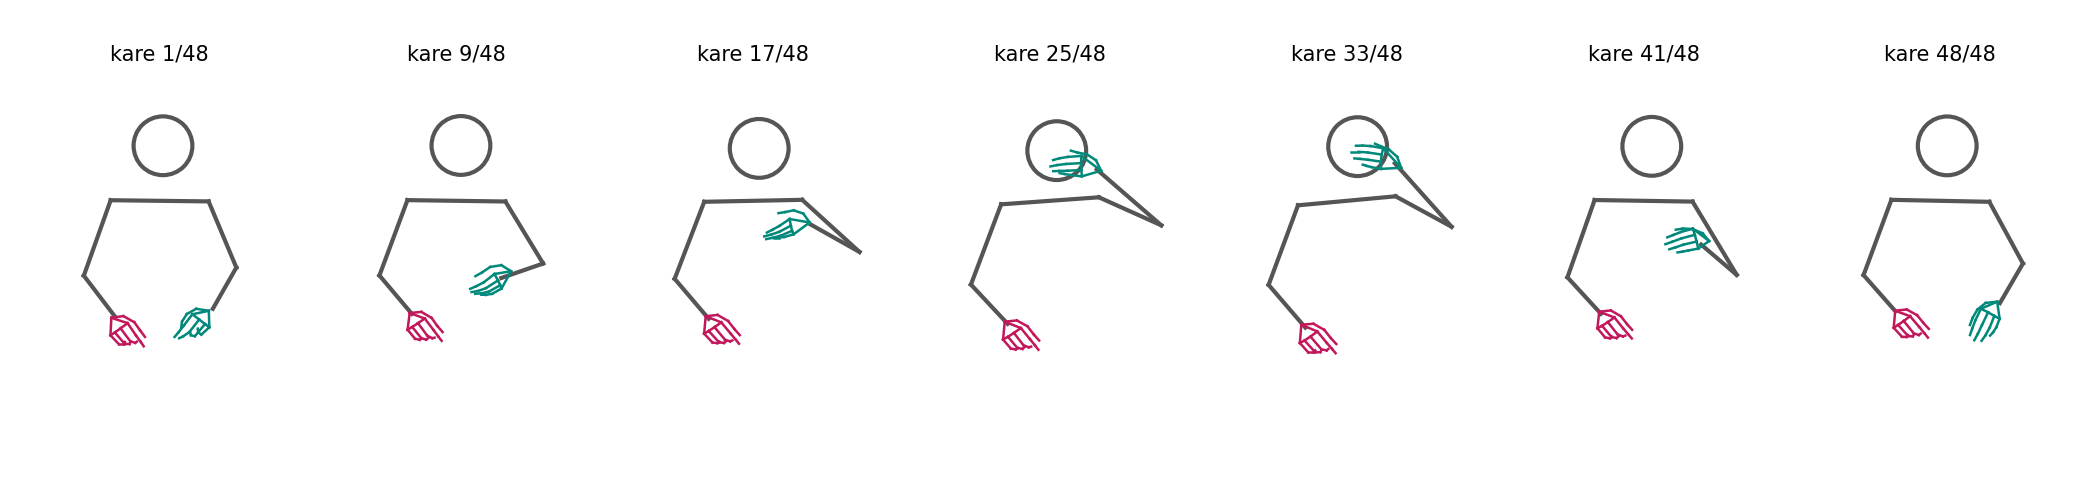
\includegraphics[width=\textwidth]{grafik/ornek_hareket.png}
\caption{\sol çorba\sag{} işaretinin örnek hareketinden kareler (eğitim kümesinden, normalize edilmiş noktalar)}
\label{fig:ornekhareket}
\end{figure}

\subsection{Sürekli tanıma}

Sürekli modda işaretin nerede başlayıp bittiğini bulmak için basit bir kural
kullanılmaktadır (\texttt{SegmentTracker}). En az bir elin bileği omuz ortasının bir
omuz genişliği altından yukarıdaysa kare \sol etkin\sag{} sayılır. Art arda iki etkin
kare görülünce bölüt açılır ve öncesindeki 8 kare başa eklenir; 600 ms boyunca etkinlik
olmazsa ya da 6 saniye dolarsa bölüt kapanıp sınıflandırılır. 12 kareden kısa bölütler
atılır. AUTSL test videoları 10 FPS'e seyreltilip bu kuralla bölütlendiğinde bulunan
bölütlerde doğruluk yüzde 89--90 olarak ölçülmüştür (\texttt{tune\_segmentation.py}).

\subsection{Gönüllü testi ekranı}

Gerçek ortam doğruluğunu ölçmek için uygulamaya ayrı bir test ekranı eklenmiştir.
Katılımcıya rastgele seçilmiş 10, 20 ya da 30 kelime sırayla gösterilir; her kelimenin
örnek hareketi ekranın üstünde oynar. Katılımcı işareti kaydeder, tahmin ve ilk üç aday
gösterilir. Her deneme yalnızca nokta koordinatları ve tahminle birlikte telefona JSON
olarak yazılır; kamera görüntüsü saklanmaz. Test sonunda Top-1, Top-3 ve eşiği geçenlerde
doğruluk özetlenir. Kayıtlar bilgisayara alınıp \texttt{live\_analysis.py} ile
incelenmektedir: betik kayıtları Python'da yeniden sınıflandırır, katılımcı bazında
doğruluk çıkarır ve canlı kayıtları AUTSL ile kare sayısı, elin görünme oranı,
kameraya uzaklık ve el hızı açısından karşılaştırır.

\subsection{Gizlilik ve çevrimdışı çalışma}

Uygulamanın Android bildiriminde (\textit{manifest}) yalnızca kamera izni
bulunmaktadır; internet izni yoktur. Model, MediaPipe dosyaları ve örnek hareketler
uygulama paketinin içindedir. Kamera görüntüsü hiçbir aşamada diske yazılmaz ve
cihazdan çıkmaz.

\subsection{Karşılaşılan sorunlar}

\begin{itemize}
  \item Yayın (\textit{release}) derlemesinde kod küçültme aracı (R8), MediaPipe'ın
        kullandığı protobuf alan adlarını değiştirdiği için uygulama açılışta
        çökmüştür. Yayın derlemesinde küçültme kapatılarak sorun giderilmiştir.
  \item Flutter'ın 3.50 sürümü projenin Gradle yapılandırmasıyla uyumsuz olduğu için
        Flutter 3.44.8 sürümüne sabitlenmiştir.
  \item Uzun video testleri ve sürekli kamera kullanımı orta segment telefonu
        ısıtmaktadır (46,7 °C ölçülmüştür). Bu nedenle CPU modu uzun süreli kullanım
        için önerilmemektedir.
\end{itemize}

\section{Değerlendirme}
\label{CH:Degerlendirme}

\subsection{Başarı ölçütlerine göre durum}

Tez önerisindeki ölçütlerin ölçülen değerleri Tablo~\ref{tab:durum} içinde
özetlenmiştir.

\begin{table}[H]
\centering
\caption{Başarı ölçütleri ve ölçülen değerler}
\label{tab:durum}
\small
\begin{tabularx}{\textwidth}{@{}l l X l@{}}
\toprule
\textbf{Ölçüt} & \textbf{Hedef} & \textbf{Ölçülen} & \textbf{Durum} \\
\midrule
Top-1 doğruluk (AUTSL test) & $\geq$ \%85 & \%89,42 $\pm$ 0,52 (3 tohum); uygulamadaki int8 model \%89,82 & Sağlandı \\
Gerçek ortam doğruluğu & $\geq$ \%75 & \olculecek{gönüllü testi, Top-1} & -- \\
Model boyutu & $\leq$ 10 MB & 1,61 MB (int8 \texttt{.tflite}) & Sağlandı \\
İşleme hızı & $\geq$ 15 FPS & Yaklaşık 9 FPS (Redmi Note 10 Pro, önceki sürüm); yeni sürüm \olculecek{FPS} & Sağlanmadı \\
İnternet bağımlılığı & Tam çalışma & İnternet izni yok; uçak modunda \olculecek{deneme} & -- \\
\bottomrule
\end{tabularx}
\end{table}

\subsection{Hız}

Kare başına süre Redmi Note 10 Pro telefonda ön kamerayla, sınıflandırma modeli
olmadan ölçülmüştür (Tablo~\ref{tab:hiz}). Sınıflandırma modelinin kendisi bir işaret
bölütü için bir kez çalıştığından kare hızını belirleyen etken iki MediaPipe modelidir.

\begin{table}[H]
\centering
\caption{Yapılandırmaya göre kare hızı (Redmi Note 10 Pro, ön kamera)}
\label{tab:hiz}
\small
\begin{tabular}{@{}lrrrr@{}}
\toprule
\textbf{Yapılandırma} & \textbf{FPS} & \textbf{Kare başına (ms)} & \textbf{El (ms)} & \textbf{Gövde (ms)} \\
\midrule
Hata ayıklama sürümü, CPU, sıralı & $\sim$5 & 200--300 & 150--180 & 70--80 \\
Hepsi GPU, paralel & 7 & 120--130 & 90--120 & $\sim$100 \\
El GPU, gövde CPU, paralel & 9 & 110--120 & 70--90 & 80--100 \\
Gövde iki karede bir (yeni) & \multicolumn{4}{c}{\olculecek{tablette}} \\
\bottomrule
\end{tabular}
\end{table}

15 FPS hedefine ulaşılamamasının nedeni, her karede iki ayrı derin ağın (el ve gövde)
çalışmasıdır. Gövdenin iki karede bir çıkarılması bu yükü azaltmaktadır. Daha ileri
iyileştirmeler için analiz görüntüsünün küçültülmesi ya da el modelinin bir önceki
karedeki el konumundan başlatılması denenebilir. Öte yandan eğitimde uygulanan zamansal
seyreltme sayesinde model 10 FPS'lik girdide de çalışmaktadır: AUTSL test videoları
10 FPS'e seyreltildiğinde doğruluk yalnızca 0,8 puan düşmektedir (BiGRU, yüzde 88,00'den
yüzde 87,22'ye).

\subsection{Kayıtlı veri ile canlı kullanım arasındaki fark}

Proje boyunca yapılan canlı denemelerde tahmin güvenlerinin kayıtlı veriye göre
belirgin biçimde düştüğü gözlenmiştir. Bu farkı ayırmak için şu denemeler yapılmıştır:

\begin{itemize}
  \item \textbf{Öz-test:} Kayıtlı noktalar telefonda sınıflandırıldığında Python ile
        yüzde 99,5 aynı tahmin alınmıştır. Yani sorun ön işleme ya da modelin
        dönüşümünde değildir.
  \item \textbf{Video dosyasından telefon çıkarımı:} AUTSL videoları kamerasız olarak
        telefondaki MediaPipe zincirinden geçirildiğinde 14 videodan 10'u doğru
        tanınmıştır (yüzde 71; aynı kliplerde Python yüzde 81,7). Telefon ısındığı için
        deneme yarıda kesilmiş, örnek sayısı az kalmıştır.
  \item \textbf{Segmentleme:} 10 FPS'e seyreltilmiş AUTSL videolarında bölütleme
        kuralı doğruluğu bozmamaktadır (yüzde 89--90).
  \item \textbf{Kullanıcının işareti bilmesi:} İlk canlı denemeleri işaret dili
        bilmeyen ekip üyeleri yapmış, bazı denemelerde sözlükte olmayan işaretler
        (örneğin harfler) denenmiştir. Örnek hareket animasyonu bu nedenle eklenmiştir.
\end{itemize}

Bu bulgular farkın büyük ölçüde girdinin kendisinden (kişinin işareti doğru yapması,
kameraya uzaklık, ışık, kamera açısı) kaynaklandığını düşündürmektedir. Gönüllü
testinde toplanan kayıtlar \texttt{live\_analysis.py} ile AUTSL'ye göre karşılaştırılarak
bu etkenler sayısal olarak ayrıştırılacaktır. Sonuç: \olculecek{gönüllü testi analizi}.

\subsection{Gönüllü testi}

Gönüllü testi Ek~\ref{EK:Gonullu} içindeki protokole göre ekip dışından katılımcılarla
yapılmaktadır. Her katılımcı uygulamadaki test ekranında rastgele seçilmiş 30 kelimeyi
örnek hareketi izledikten sonra kameraya yapmaktadır.

\begin{table}[H]
\centering
\caption{Gönüllü testi sonuçları}
\label{tab:gonullu}
\begin{tabular}{@{}lrrr@{}}
\toprule
\textbf{Katılımcı} & \textbf{Deneme} & \textbf{Top-1 (\%)} & \textbf{Top-3 (\%)} \\
\midrule
\multicolumn{4}{c}{\olculecek{katılımcı sonuçları}} \\
\bottomrule
\end{tabular}
\end{table}

\section{Sonuç ve Gelecek Çalışmalar}
\label{CH:Sonuc}

Bu projede telefon kamerasıyla Türk İşaret Dili kelimelerini tanıyan, internetsiz
çalışan bir Android uygulaması geliştirilmiştir. AUTSL veri setinin işaretçiden
bağımsız bölmelerinde iki model karşılaştırılmış; 1B-CNN + Transformer modeli üç
tohumda yüzde $89{,}42 \pm 0{,}52$ test doğruluğuyla BiGRU'yu (yüzde
$87{,}98 \pm 0{,}23$) geride bırakmış ve daha az parametreyle yüzde 85 hedefini
aşmıştır. Model int8 LiteRT biçiminde 1,61 MB'tır ve dönüşüm doğruluğu
düşürmemiştir. Eğitim ve uygulama tarafında aynı MediaPipe modelleri ve birebir aynı
ön işleme kullanıldığı için telefon ve Python tahminleri neredeyse tamamen
örtüşmektedir.

Uygulama tez önerisindeki üç ekranı içermektedir. Bunlara ek olarak her kelimenin
örnek hareketini gösteren iskelet animasyonu ve gerçek ortam doğruluğunu ölçmek için
gönüllü testi ekranı eklenmiştir. Model boyutu ve AUTSL doğruluğu hedefleri
sağlanmış, internet bağlantısı gerektirmeyen bir yapı kurulmuştur. Uçtan uca hız ise
iki MediaPipe modelinin kare başına çalışması nedeniyle 15 FPS hedefinin altında
kalmıştır.

\subsection*{Gelecek çalışmalar}

\begin{itemize}
  \item \textbf{Canlı veriyle ince ayar:} Gönüllü testinde toplanan nokta kayıtları
        eğitim kümesine eklenerek model telefon kamerası koşullarına uyarlanabilir.
  \item \textbf{Sözlüğün genişletilmesi:} BosphorusSign22k (744 işaret) ve
        TurkSign446 (446 işaret) veri setlerine erişim izni alınarak sözlük
        büyütülebilir. TurkSign446 noktaları MediaPipe ile çıkarıldığı için mevcut
        hatta görece kolay eklenebilir.
  \item \textbf{Hız:} Analiz görüntüsünün küçültülmesi, el izlemenin önceki kareden
        başlatılması ve gövde modelinin daha seyrek çalıştırılması ile 15 FPS hedefine
        yaklaşılabilir.
  \item \textbf{Ayırt edici bilgi:} En çok karışan işaretler parmak teması ve derinlik
        bilgisiyle ayrışmaktadır. Elin derinlik koordinatı ve yüz noktalarının girdiye
        eklenmesi bu hataları azaltabilir.
  \item \textbf{Cümle düzeyi:} Ardışık kelimelerin dilbilgisel Türkçe cümleye
        çevrilmesi, sürekli işaret dili veri setleriyle ele alınabilir.
\end{itemize}


\bibliographystyle{erciyesbm}
\bibliography{referanslar}

\clearpage
\appendix
\section{Gönüllü Testi Protokolü ve Bilgilendirilmiş Onam Formu}
\label{EK:Gonullu}

\subsection*{Amaç}

Uygulamanın gerçek kullanım koşullarında (telefon kamerası, farklı kişiler, farklı
ortamlar) işaretleri ne kadar doğru tanıdığını ölçmek. Hedef, tez önerisindeki
\sol gerçek ortam doğruluğu yüzde 75\sag{} ölçütüdür.

\subsection*{Katılımcılar}

Ekip dışından, 18 yaşını doldurmuş gönüllüler. İşaret dili bilmek şart değildir;
her işaretin örnek hareketi uygulamada gösterilir. Katılımcı adı hiçbir yere yazılmaz,
yalnızca bir kod (K01, K02, \ldots) kullanılır.

\subsection*{Düzenek}

\begin{itemize}
  \item Telefon ya da tablet sabit bir yere, göğüs hizasında ve yaklaşık 1--1,5 metre
        uzağa konur. Baş, omuzlar ve iki el görüntüde olmalıdır.
  \item Ön kamera kullanılır. Ortam ışığı not edilir (gün ışığı / yapay ışık).
  \item Uygulama uçak modunda çalıştırılır.
\end{itemize}

\subsection*{Uygulama}

\begin{enumerate}
  \item İşaretler sekmesinde sağ üstteki \sol Gönüllü testi\sag{} açılır, katılımcı
        kodu girilir ve 30 işaret seçilir.
  \item Her kelime için katılımcı örnek hareketi en az iki kez izler, \sol Kaydet\sag{}
        düğmesine basar, işareti yapar ve \sol Bitir\sag{} düğmesine basar.
  \item Kayıt hatalıysa (el görünmedi, çok kısa) bir kez yeniden kaydedilir; tahmin
        çıktıysa \sol Sonraki\sag{} ile devam edilir. Yanlış tahminde yeniden deneme
        yapılmaz.
  \item Test sonunda özet ekranı kaydedilir (ekran görüntüsü).
  \item Kayıtlar bilgisayara alınır ve \texttt{python ml/live\_analysis.py} ile incelenir:\\
        {\small\texttt{adb pull /sdcard/Android/data/tr.edu.erciyes.tid\_app/\\files/gonullu\_testi}}
\end{enumerate}

\subsection*{Saklanan veri}

Her deneme için yalnızca el ve gövde noktalarının koordinatları, hedef kelime,
modelin ilk üç tahmini, güven değerleri ve katılımcı kodu saklanır. Kamera görüntüsü
ve ses kaydedilmez. Veriler yalnızca bu bitirme projesi kapsamında kullanılır ve proje
bitiminde silinir.

\subsection*{Bilgilendirilmiş onam formu}

\noindent Erciyes Üniversitesi Bilgisayar Mühendisliği Bölümü bitirme projesi
\sol MediaPipe ve Makine Öğrenmesi Kullanarak Türk İşaret Dili Tabanlı Gerçek Zamanlı El
Hareketi Tanıma ve Çeviri Sistemi\sag{} kapsamında yapılan teste gönüllü olarak
katılıyorum. Testte telefon kamerası önünde işaret dili hareketleri yapacağımı;
görüntümün kaydedilmeyeceğini, yalnızca el ve gövde noktalarının koordinatlarının
adım yazılmadan saklanacağını; verilerin yalnızca bu proje için kullanılıp proje
sonunda silineceğini ve testi istediğim an bırakabileceğimi biliyorum.

\vspace{1cm}
\noindent
\begin{tabular}{@{}p{0.45\textwidth}p{0.45\textwidth}@{}}
Katılımcı kodu: \dotfill & Tarih: \dotfill \\[8mm]
İmza: \dotfill & Testi yürüten: \dotfill \\
\end{tabular}


\end{document}
